\begin{figure}[t]
\centering
	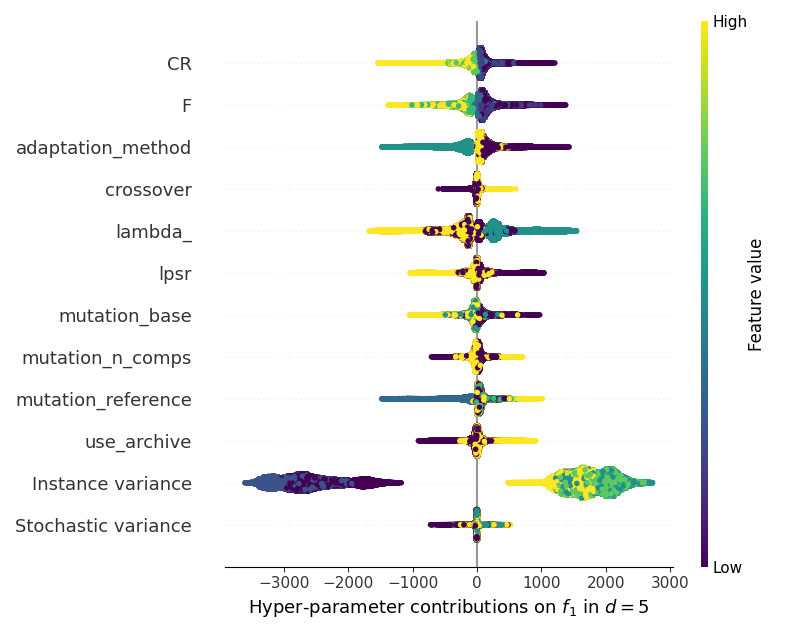
\includegraphics[height=0.15\textheight,trim=0mm 0mm 30mm 0mm,clip]{de_img_new/img_summary_f1_d5.png}
	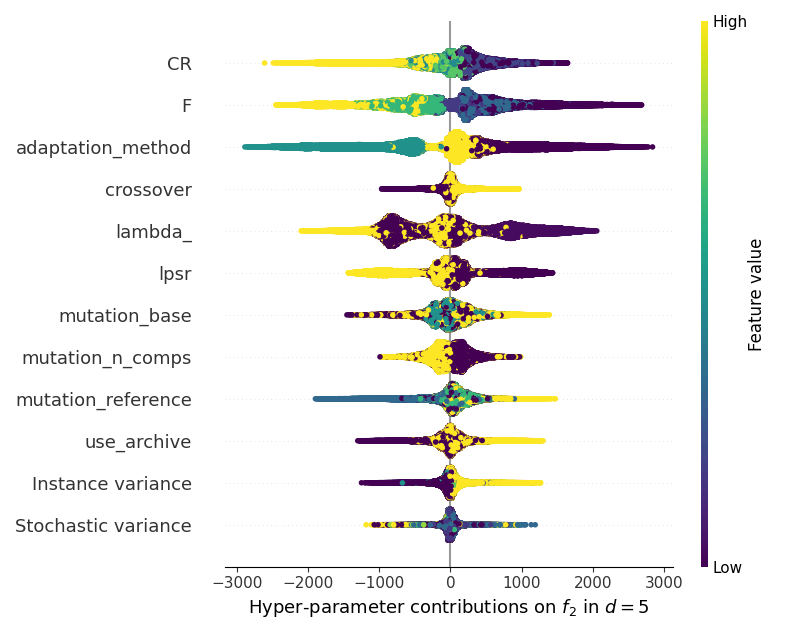
\includegraphics[height=0.15\textheight,trim=60mm 0mm 30mm 0mm,clip]{de_img_new/img_summary_f2_d5.png}
	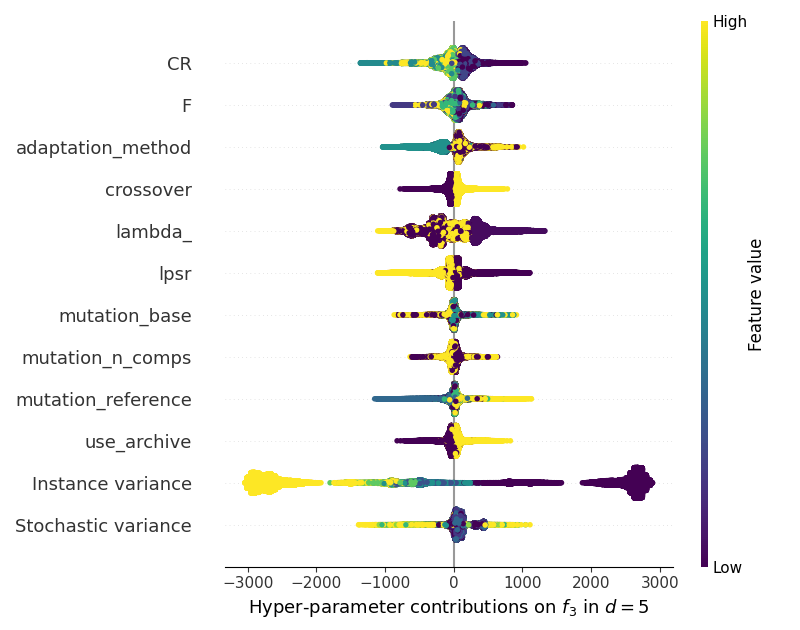
\includegraphics[height=0.15\textheight,trim=60mm 0mm 30mm 0mm,clip]{de_img_new/img_summary_f3_d5.png}
	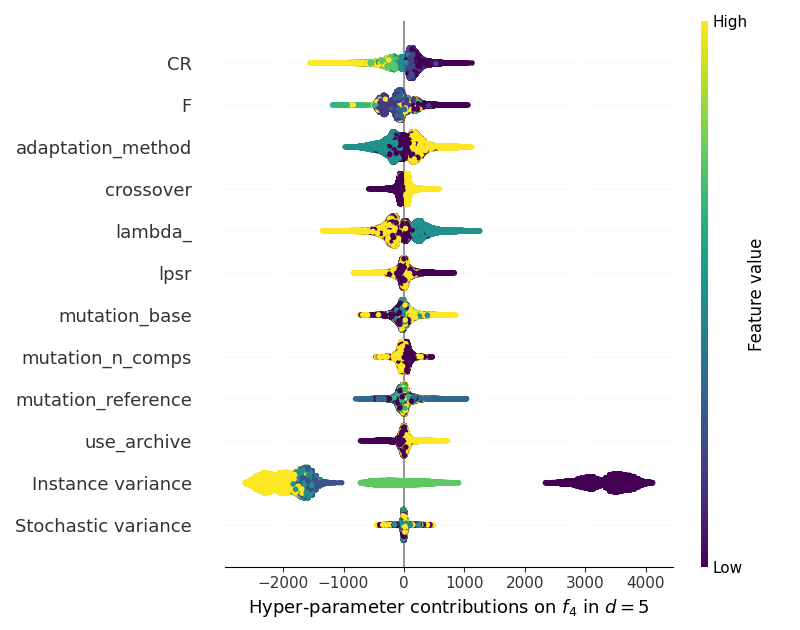
\includegraphics[height=0.15\textheight,trim=60mm 0mm 0mm 0mm,clip]{de_img_new/img_summary_f4_d5.png}
	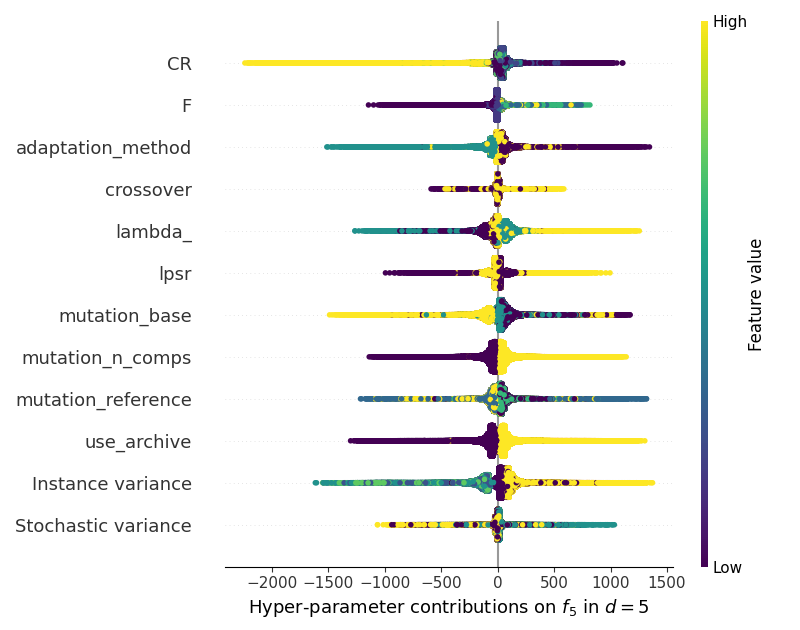
\includegraphics[height=0.15\textheight,trim=0mm 0mm 30mm 0mm,clip]{de_img_new/img_summary_f5_d5.png}
	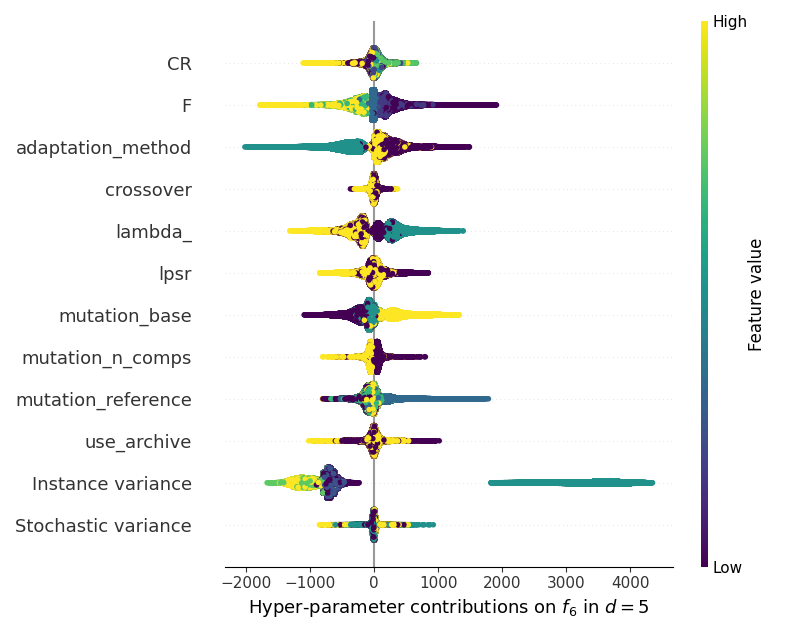
\includegraphics[height=0.15\textheight,trim=60mm 0mm 30mm 0mm,clip]{de_img_new/img_summary_f6_d5.png}
	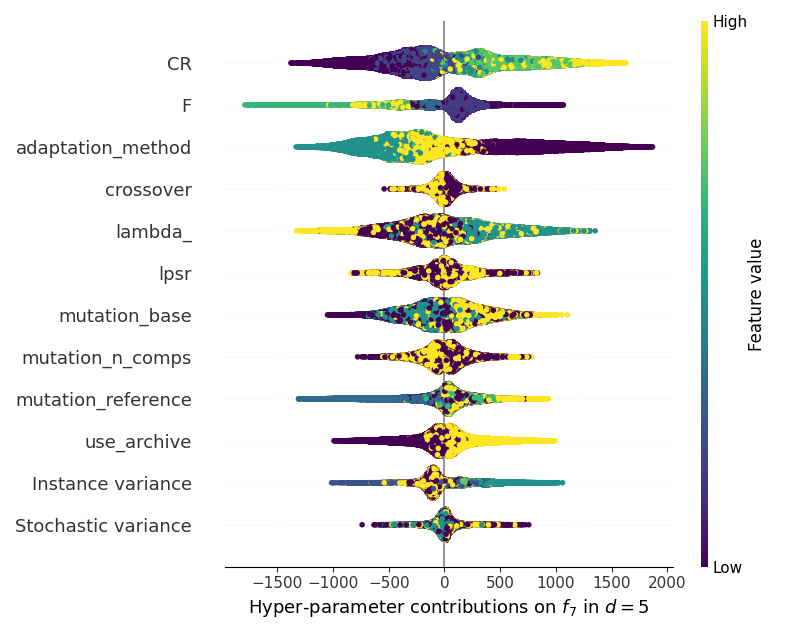
\includegraphics[height=0.15\textheight,trim=60mm 0mm 30mm 0mm,clip]{de_img_new/img_summary_f7_d5.png}
	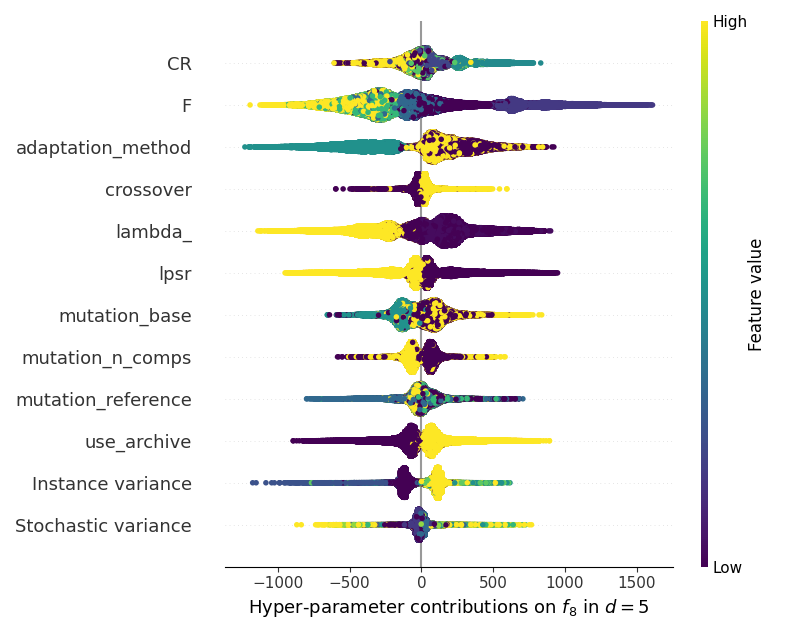
\includegraphics[height=0.15\textheight,trim=60mm 0mm 0mm 0mm,clip]{de_img_new/img_summary_f8_d5.png}
	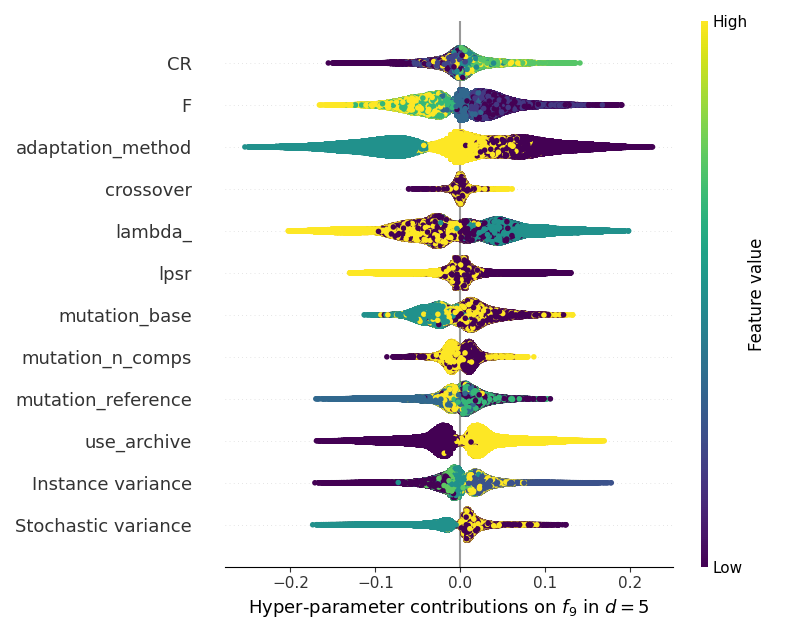
\includegraphics[height=0.15\textheight,trim=0mm 0mm 30mm 0mm,clip]{de_img_new/img_summary_f9_d5.png}
	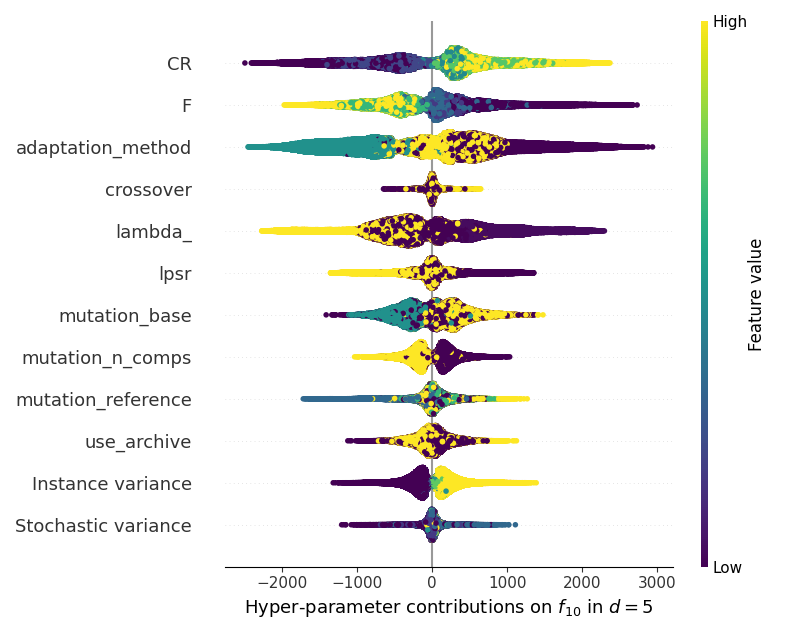
\includegraphics[height=0.15\textheight,trim=60mm 0mm 30mm 0mm,clip]{de_img_new/img_summary_f10_d5.png}
	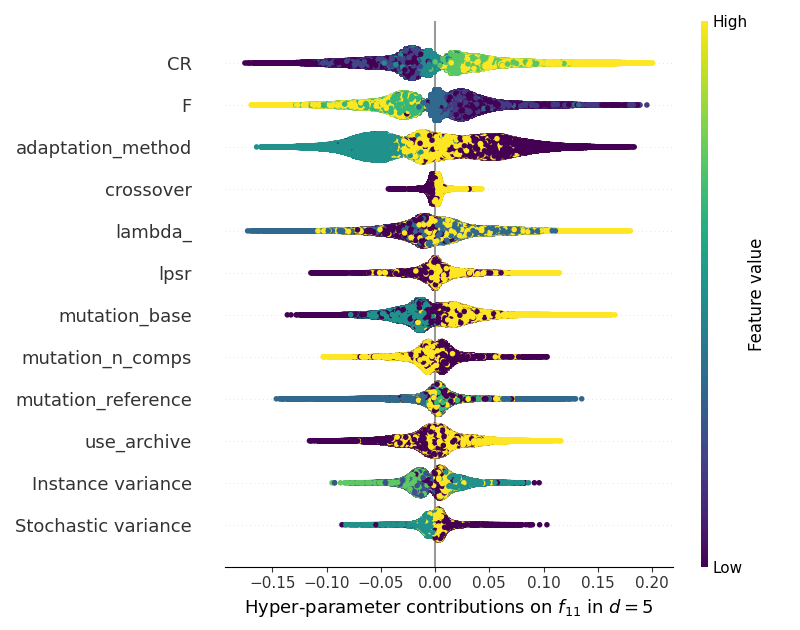
\includegraphics[height=0.15\textheight,trim=60mm 0mm 30mm 0mm,clip]{de_img_new/img_summary_f11_d5.png}
	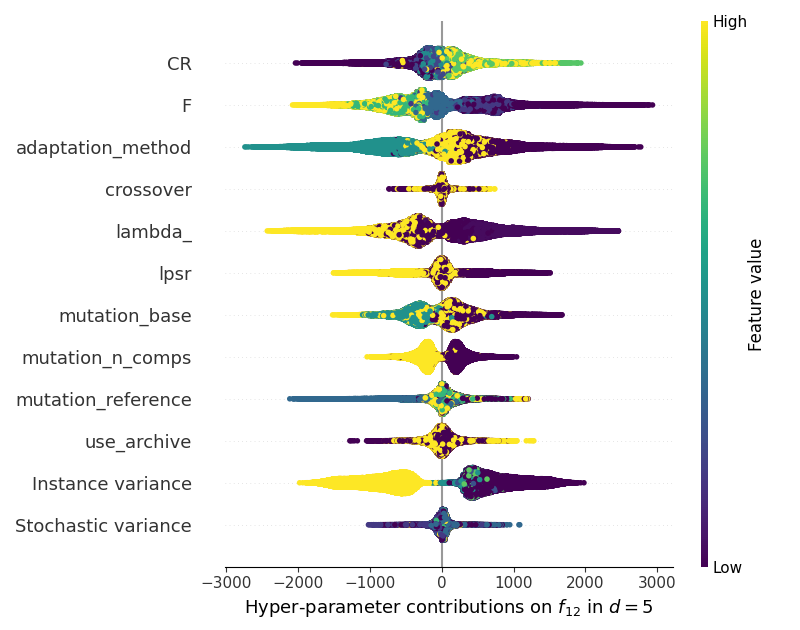
\includegraphics[height=0.15\textheight,trim=60mm 0mm 0mm 0mm,clip]{de_img_new/img_summary_f12_d5.png}
	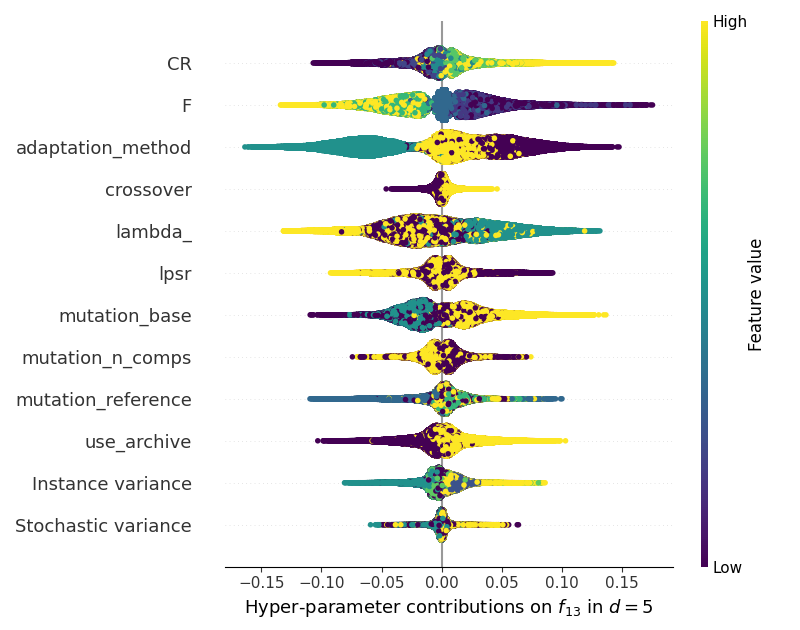
\includegraphics[height=0.15\textheight,trim=0mm 0mm 30mm 0mm,clip]{de_img_new/img_summary_f13_d5.png}
	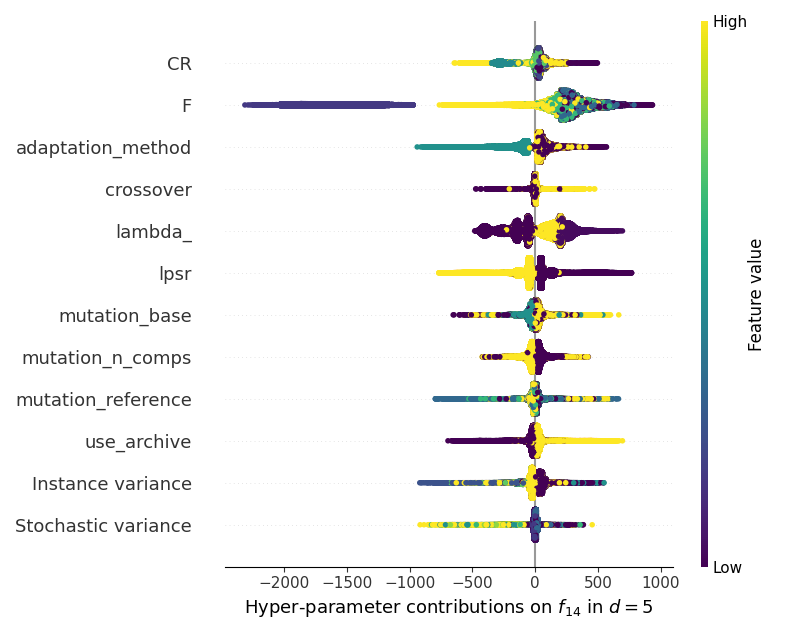
\includegraphics[height=0.15\textheight,trim=60mm 0mm 30mm 0mm,clip]{de_img_new/img_summary_f14_d5.png}
	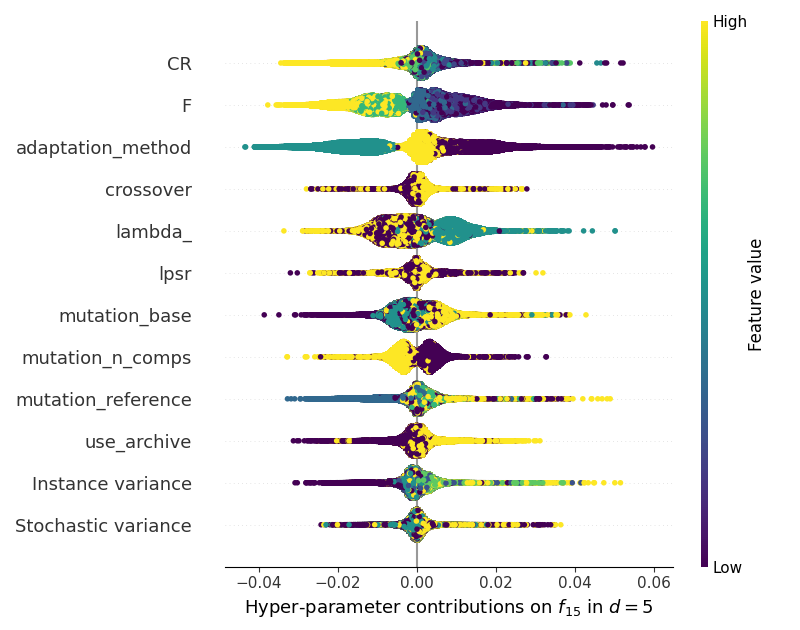
\includegraphics[height=0.15\textheight,trim=60mm 0mm 30mm 0mm,clip]{de_img_new/img_summary_f15_d5.png}
	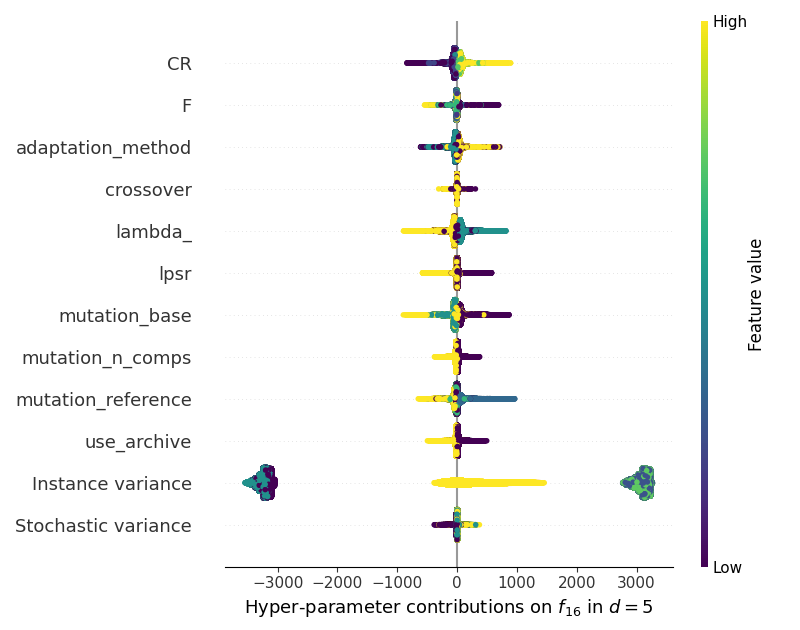
\includegraphics[height=0.15\textheight,trim=60mm 0mm 0mm 0mm,clip]{de_img_new/img_summary_f16_d5.png}
	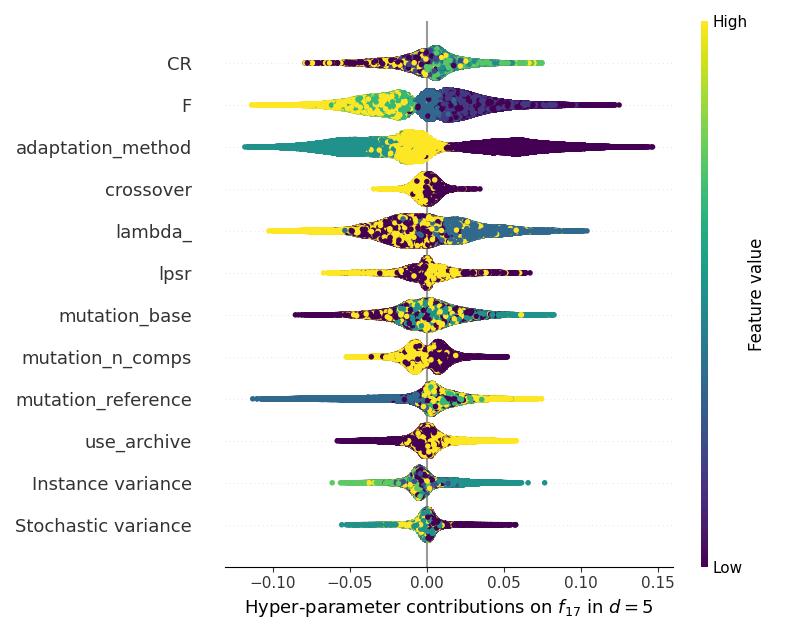
\includegraphics[height=0.15\textheight,trim=0mm 0mm 30mm 0mm,clip]{de_img_new/img_summary_f17_d5.png}
	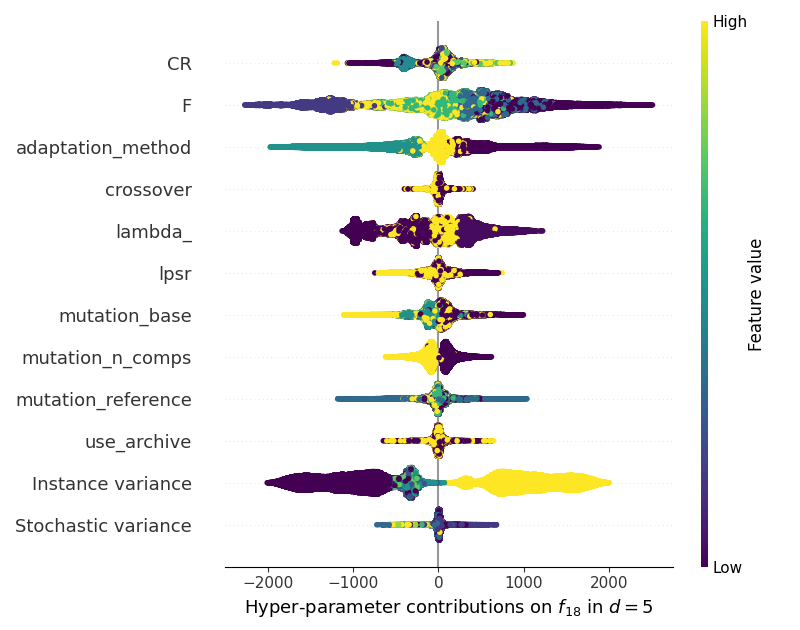
\includegraphics[height=0.15\textheight,trim=60mm 0mm 30mm 0mm,clip]{de_img_new/img_summary_f18_d5.png}
	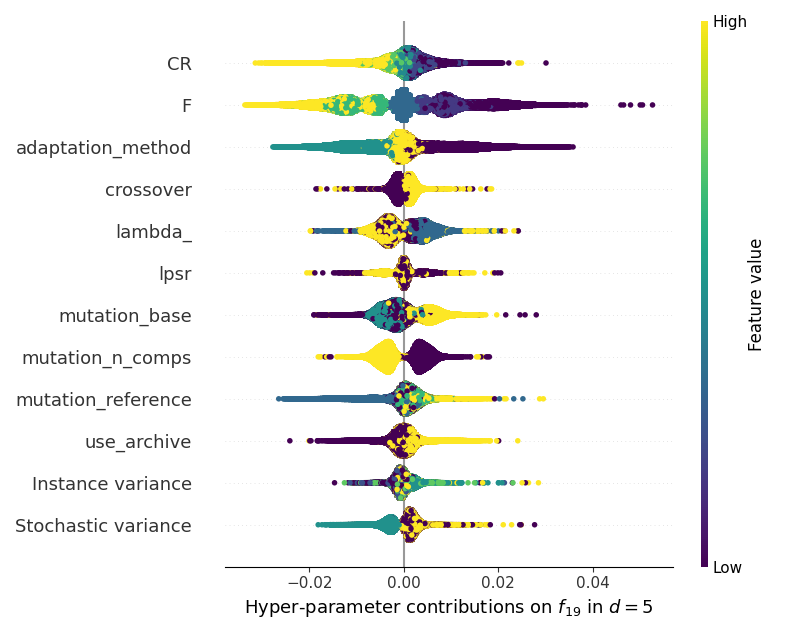
\includegraphics[height=0.15\textheight,trim=60mm 0mm 30mm 0mm,clip]{de_img_new/img_summary_f19_d5.png}
	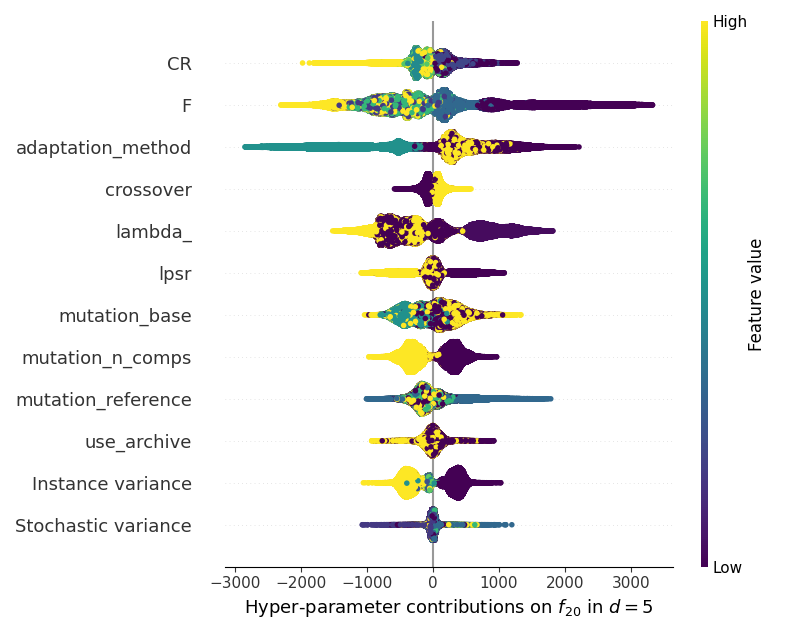
\includegraphics[height=0.15\textheight,trim=60mm 0mm 0mm 0mm,clip]{de_img_new/img_summary_f20_d5.png}
	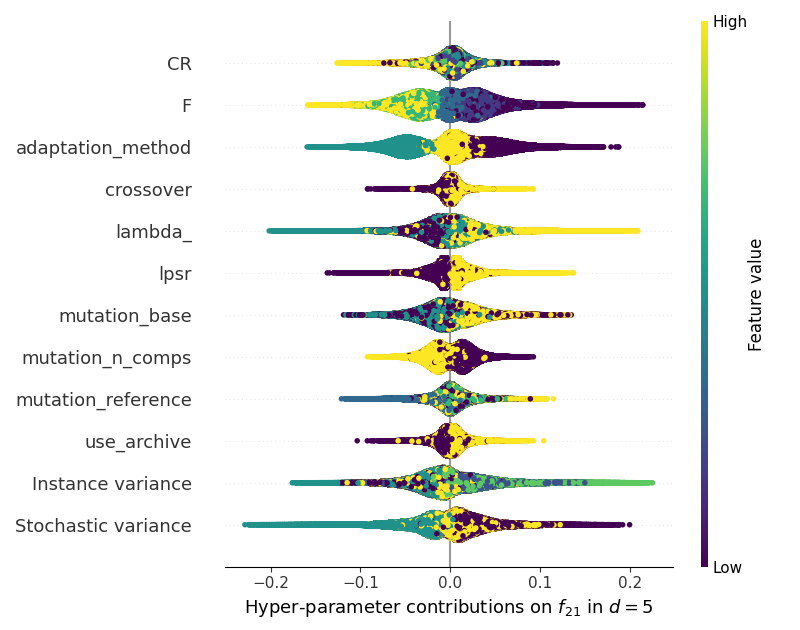
\includegraphics[height=0.15\textheight,trim=0mm 0mm 30mm 0mm,clip]{de_img_new/img_summary_f21_d5.png}
	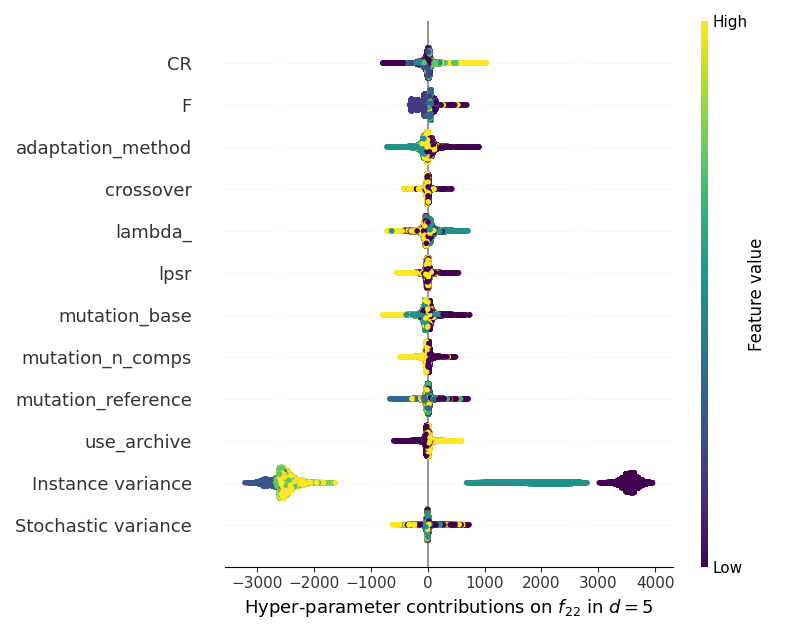
\includegraphics[height=0.15\textheight,trim=60mm 0mm 30mm 0mm,clip]{de_img_new/img_summary_f22_d5.png}
	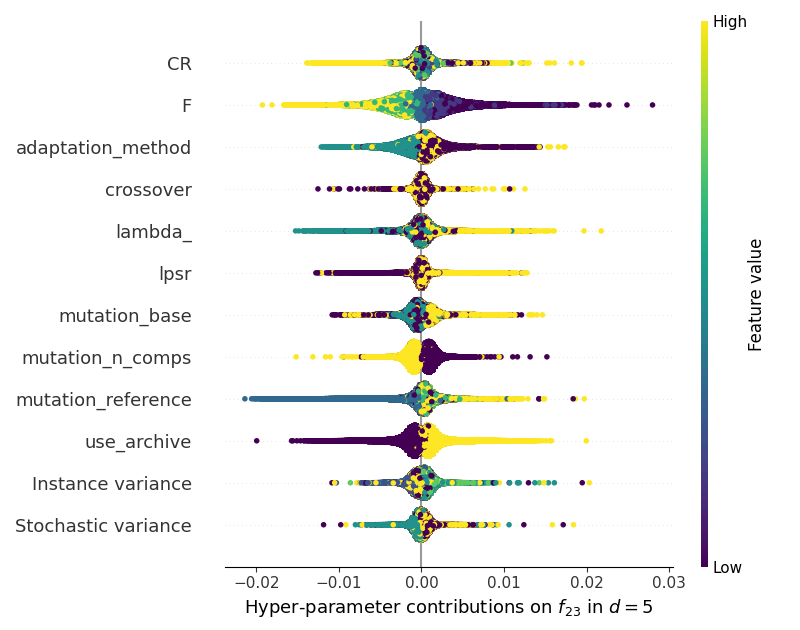
\includegraphics[height=0.15\textheight,trim=60mm 0mm 30mm 0mm,clip]{de_img_new/img_summary_f23_d5.png}
	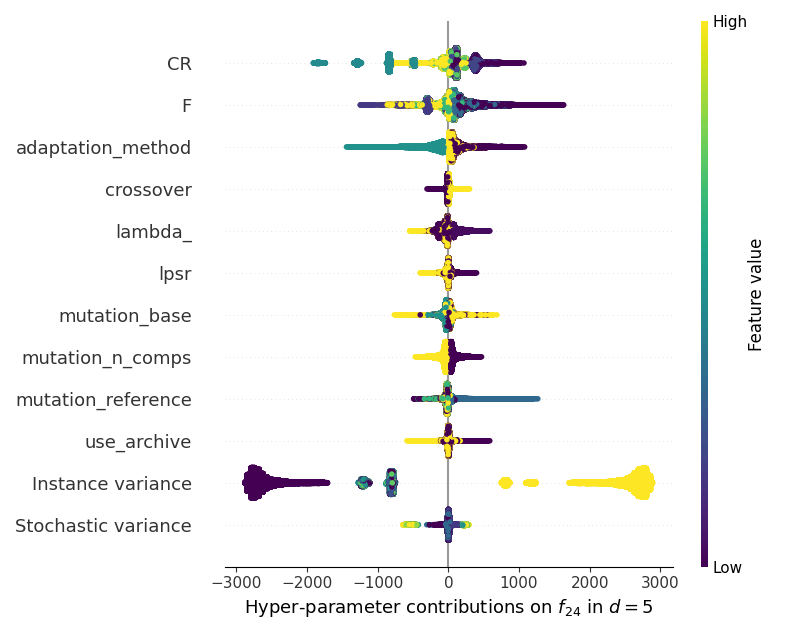
\includegraphics[height=0.15\textheight,trim=60mm 0mm 0mm 0mm,clip]{de_img_new/img_summary_f24_d5.png}
\caption{Hyper-parameter contributions per benchmark function for d=5. \label{fig:shapxplaind5}}

\end{figure}

\begin{figure}[t]
\centering
	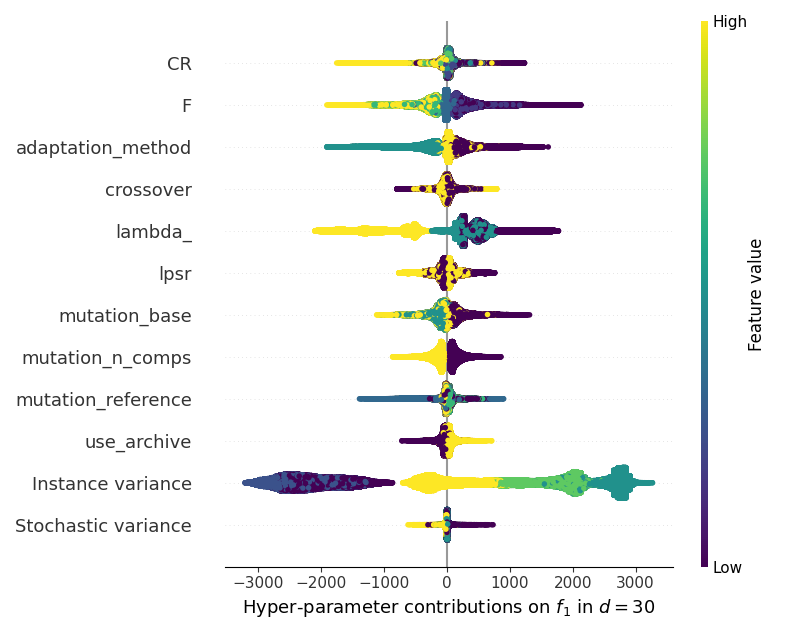
\includegraphics[height=0.15\textheight,trim=0mm 0mm 30mm 0mm,clip]{de_img_new/img_summary_f1_d30.png}
	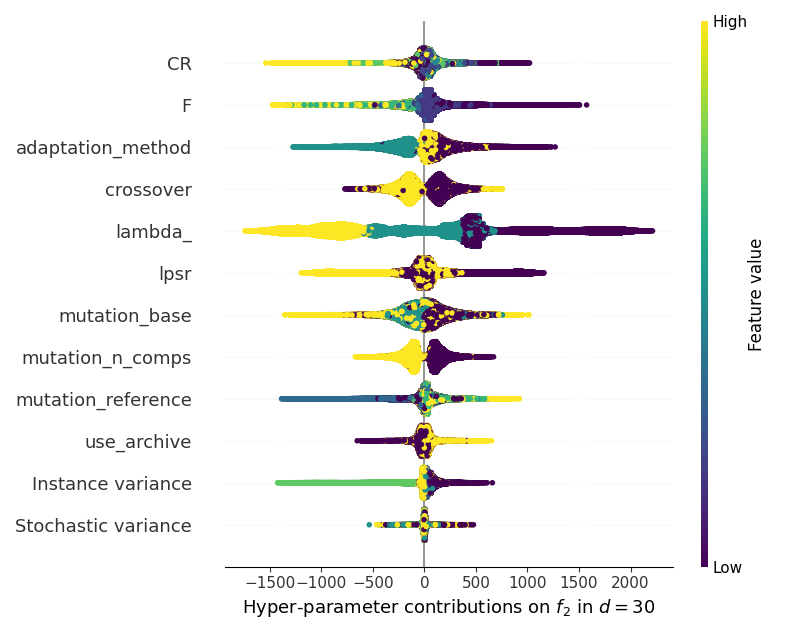
\includegraphics[height=0.15\textheight,trim=60mm 0mm 30mm 0mm,clip]{de_img_new/img_summary_f2_d30.png}
	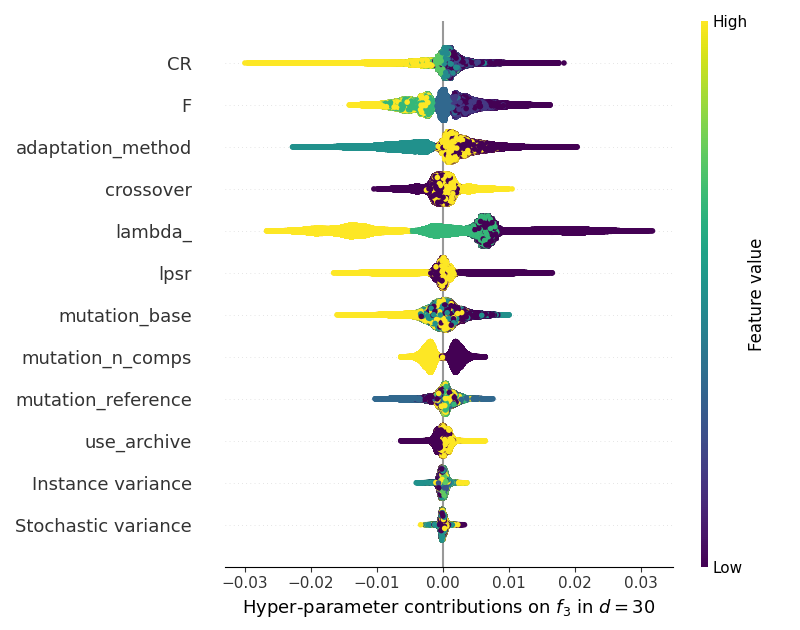
\includegraphics[height=0.15\textheight,trim=60mm 0mm 30mm 0mm,clip]{de_img_new/img_summary_f3_d30.png}
	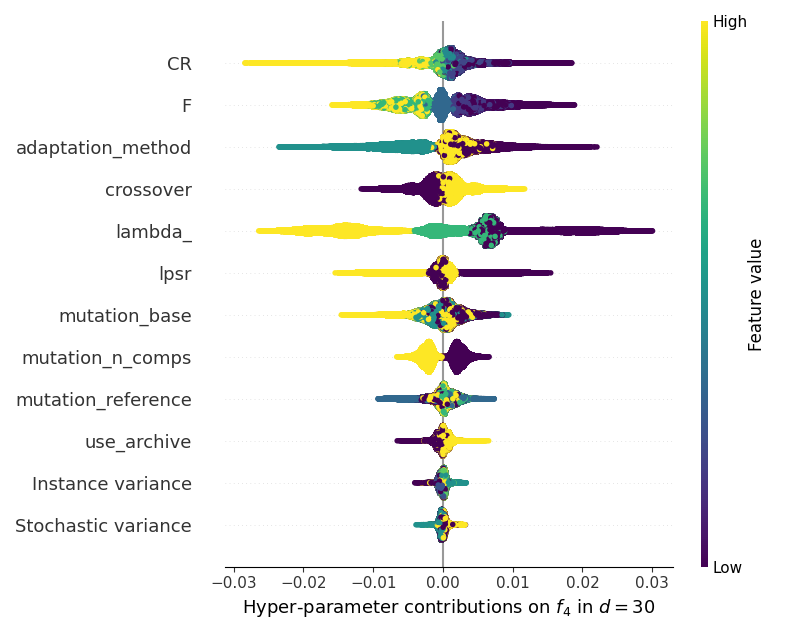
\includegraphics[height=0.15\textheight,trim=60mm 0mm 0mm 0mm,clip]{de_img_new/img_summary_f4_d30.png}
	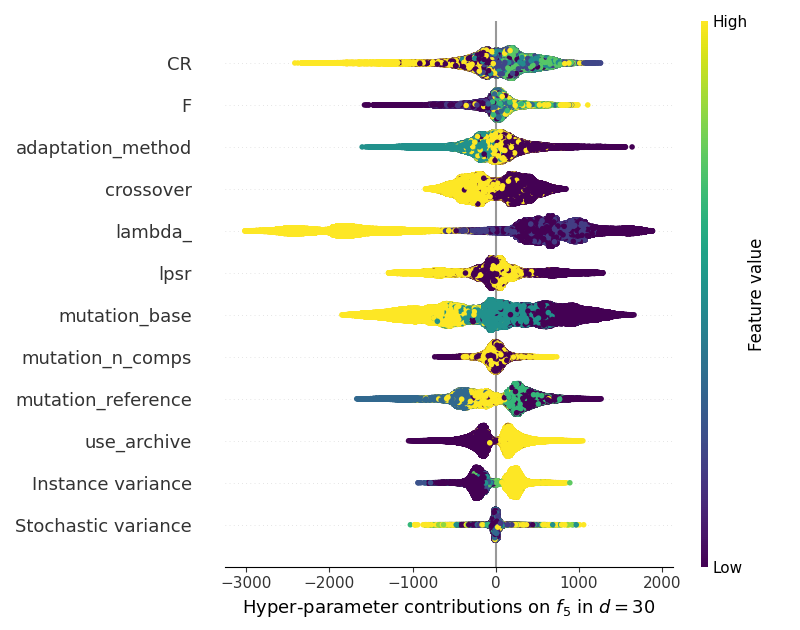
\includegraphics[height=0.15\textheight,trim=0mm 0mm 30mm 0mm,clip]{de_img_new/img_summary_f5_d30.png}
	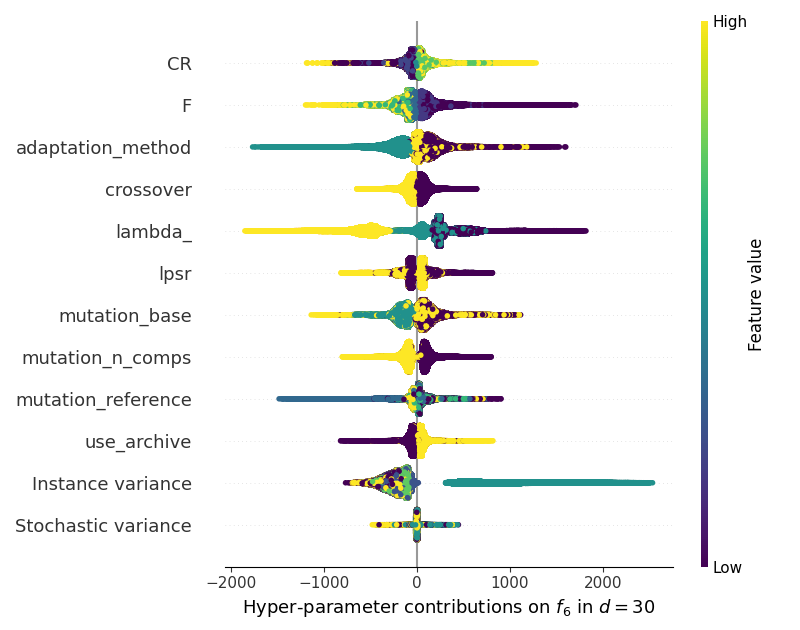
\includegraphics[height=0.15\textheight,trim=60mm 0mm 30mm 0mm,clip]{de_img_new/img_summary_f6_d30.png}
	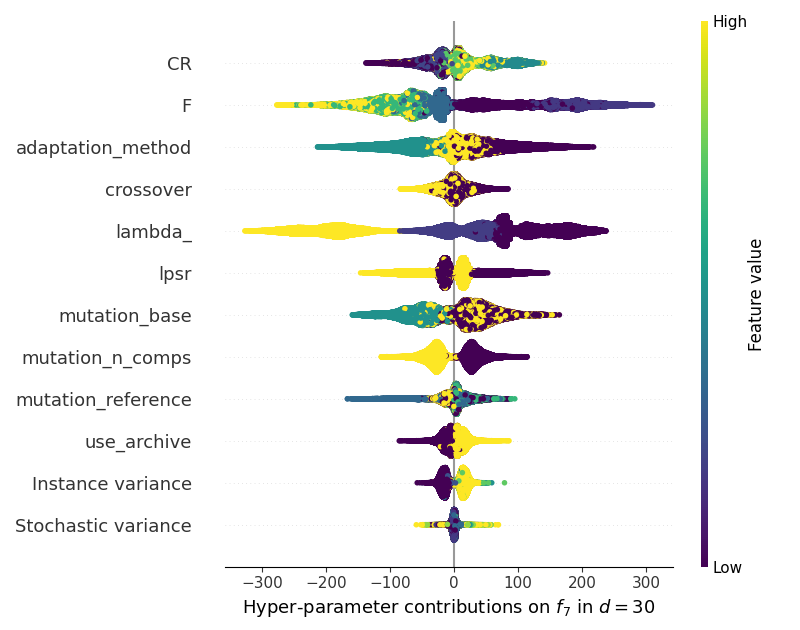
\includegraphics[height=0.15\textheight,trim=60mm 0mm 30mm 0mm,clip]{de_img_new/img_summary_f7_d30.png}
	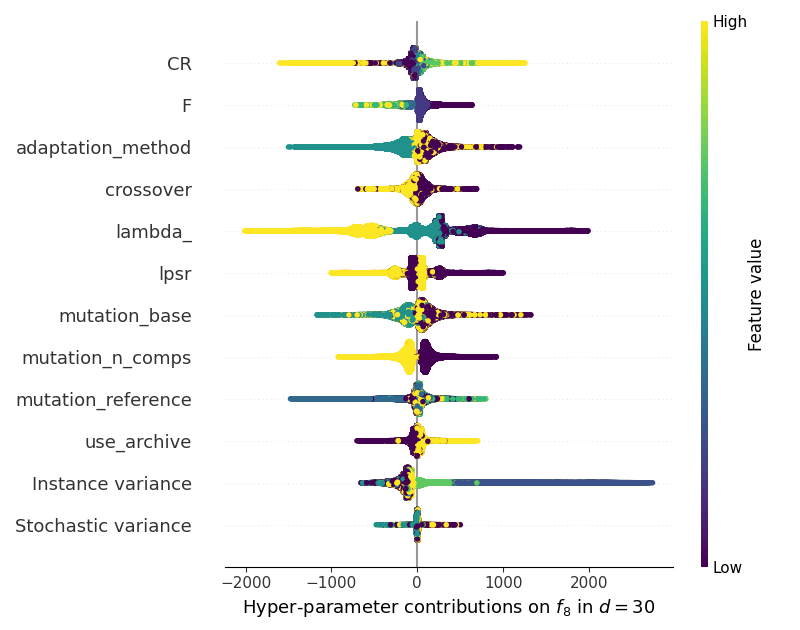
\includegraphics[height=0.15\textheight,trim=60mm 0mm 0mm 0mm,clip]{de_img_new/img_summary_f8_d30.png}
	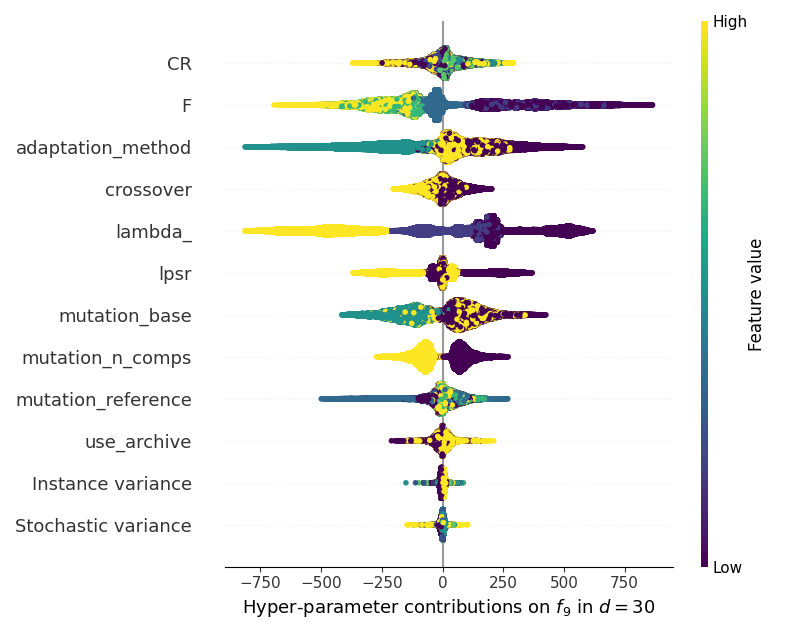
\includegraphics[height=0.15\textheight,trim=0mm 0mm 30mm 0mm,clip]{de_img_new/img_summary_f9_d30.png}
	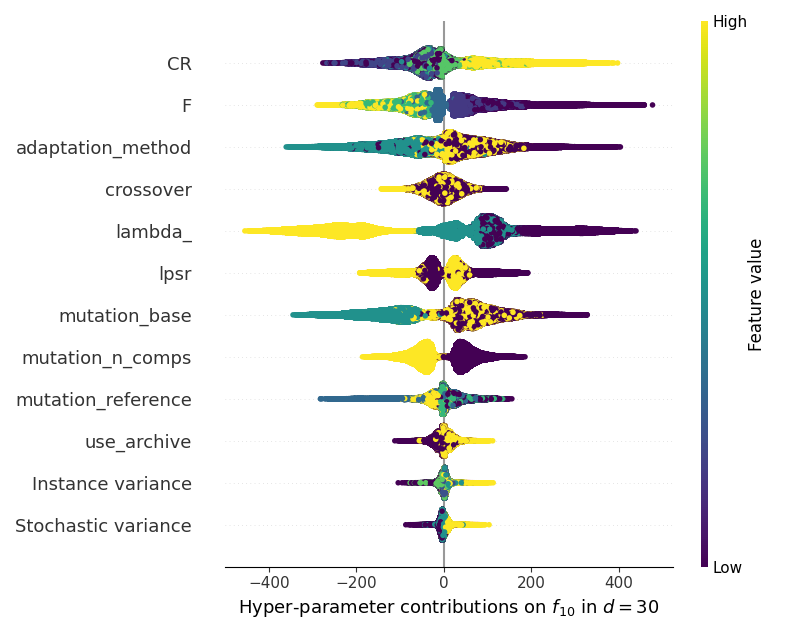
\includegraphics[height=0.15\textheight,trim=60mm 0mm 30mm 0mm,clip]{de_img_new/img_summary_f10_d30.png}
	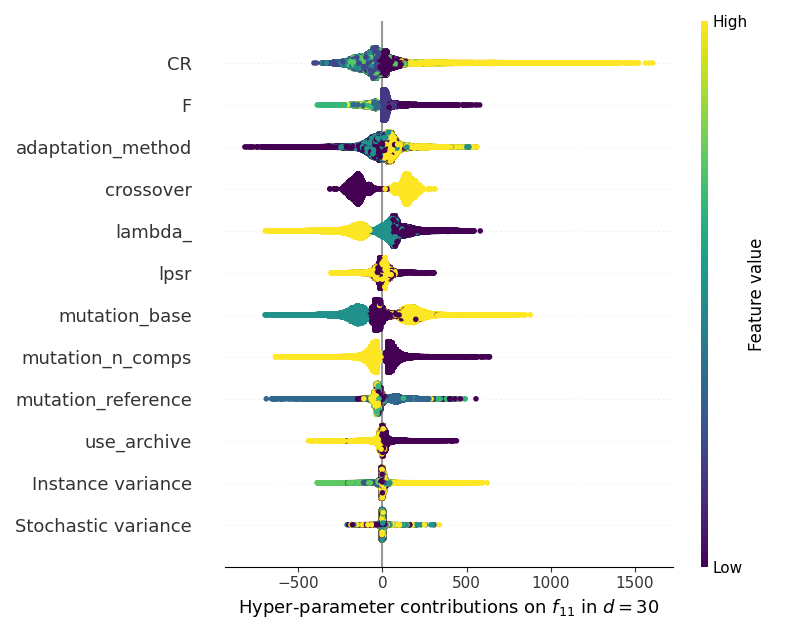
\includegraphics[height=0.15\textheight,trim=60mm 0mm 30mm 0mm,clip]{de_img_new/img_summary_f11_d30.png}
	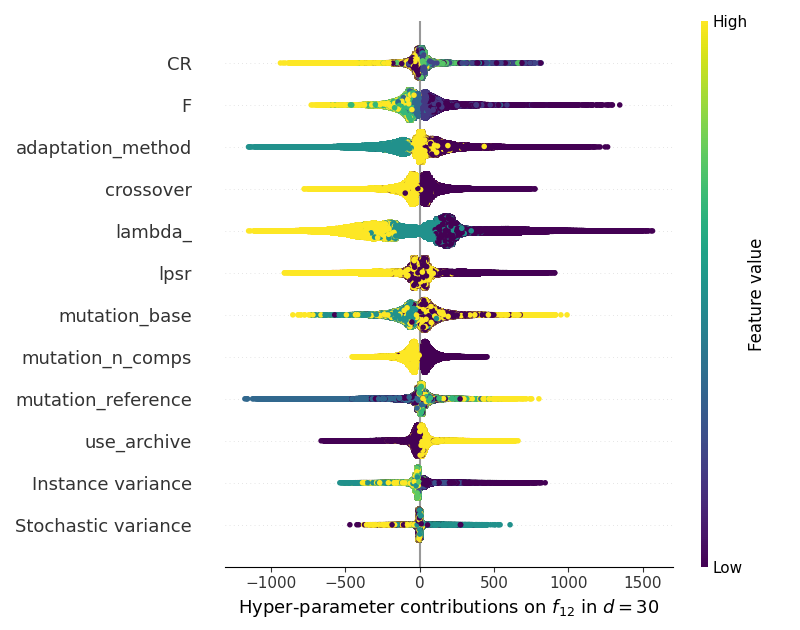
\includegraphics[height=0.15\textheight,trim=60mm 0mm 0mm 0mm,clip]{de_img_new/img_summary_f12_d30.png}
	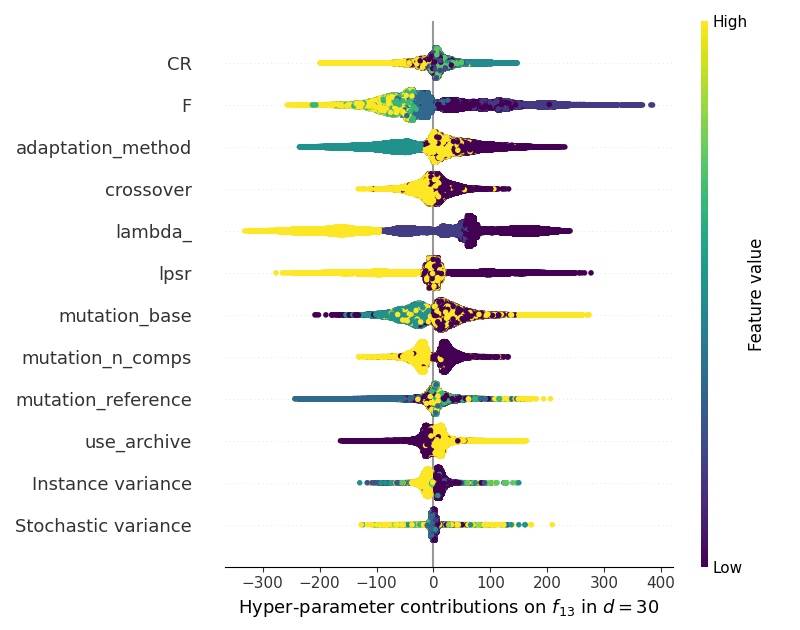
\includegraphics[height=0.15\textheight,trim=0mm 0mm 30mm 0mm,clip]{de_img_new/img_summary_f13_d30.png}
	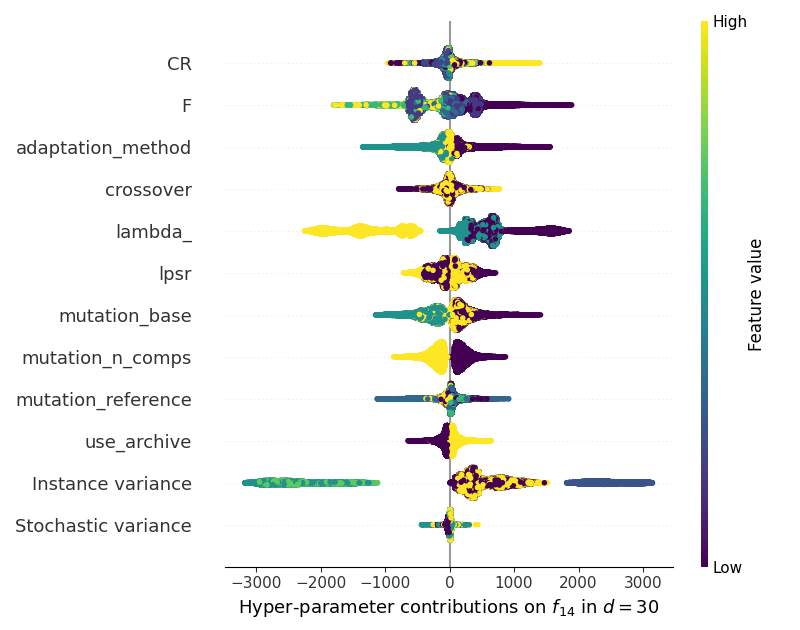
\includegraphics[height=0.15\textheight,trim=60mm 0mm 30mm 0mm,clip]{de_img_new/img_summary_f14_d30.png}
	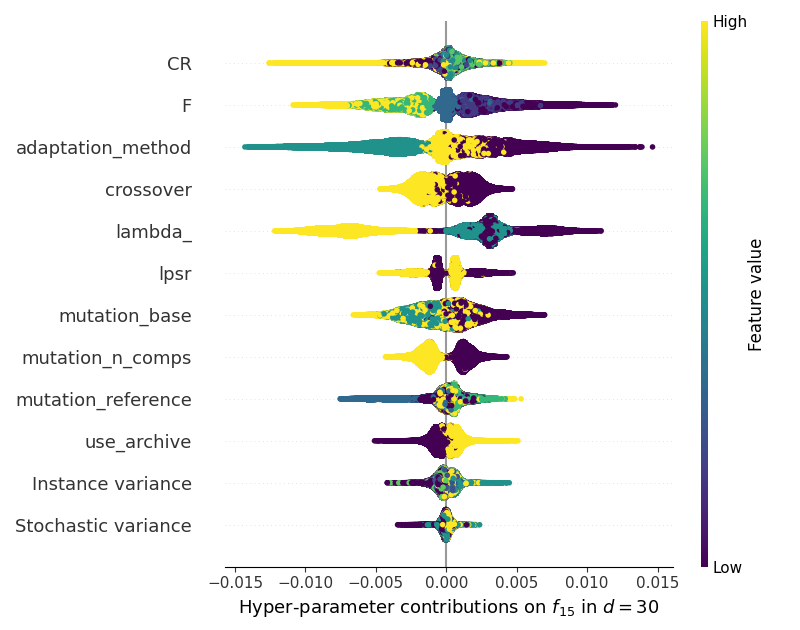
\includegraphics[height=0.15\textheight,trim=60mm 0mm 30mm 0mm,clip]{de_img_new/img_summary_f15_d30.png}
	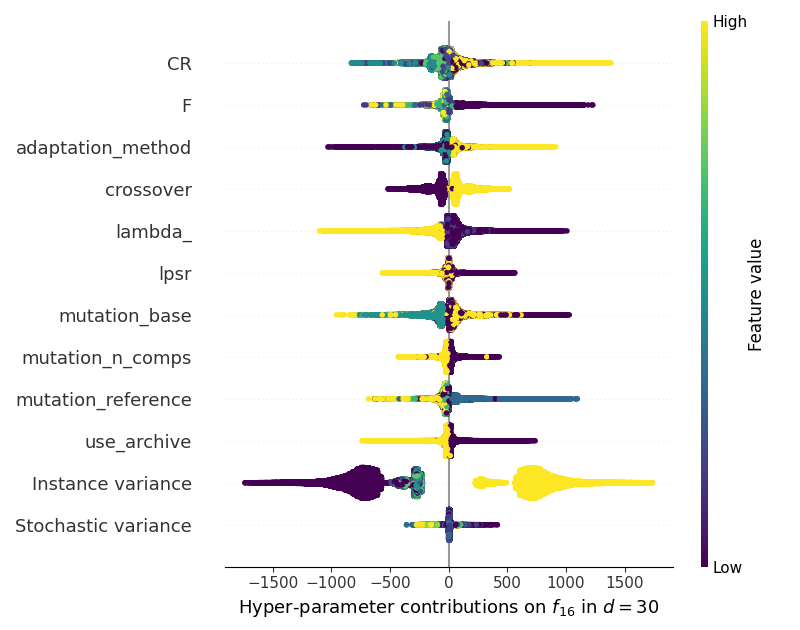
\includegraphics[height=0.15\textheight,trim=60mm 0mm 0mm 0mm,clip]{de_img_new/img_summary_f16_d30.png}
	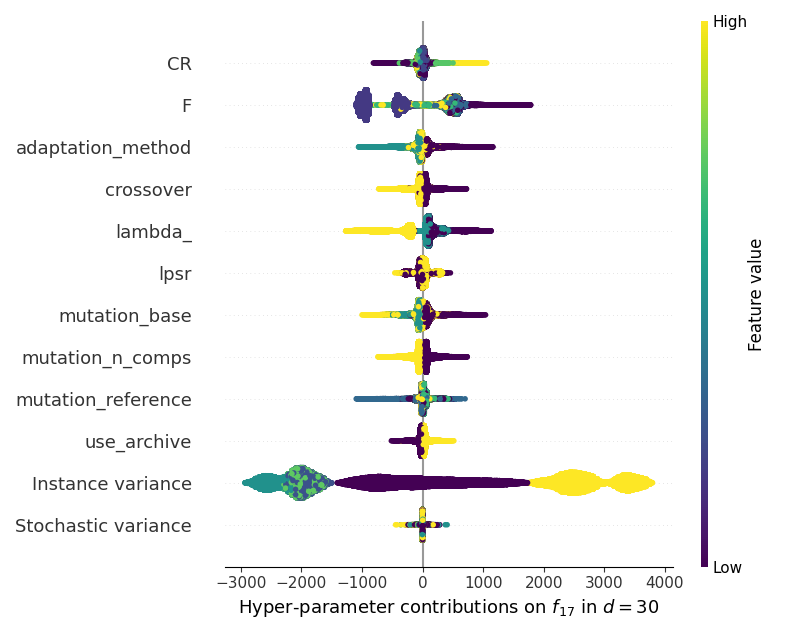
\includegraphics[height=0.15\textheight,trim=0mm 0mm 30mm 0mm,clip]{de_img_new/img_summary_f17_d30.png}
	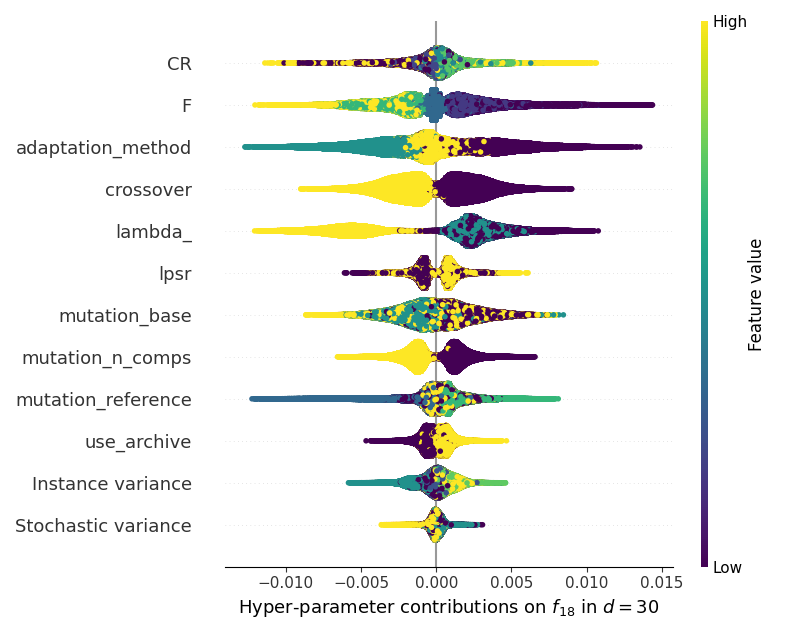
\includegraphics[height=0.15\textheight,trim=60mm 0mm 30mm 0mm,clip]{de_img_new/img_summary_f18_d30.png}
	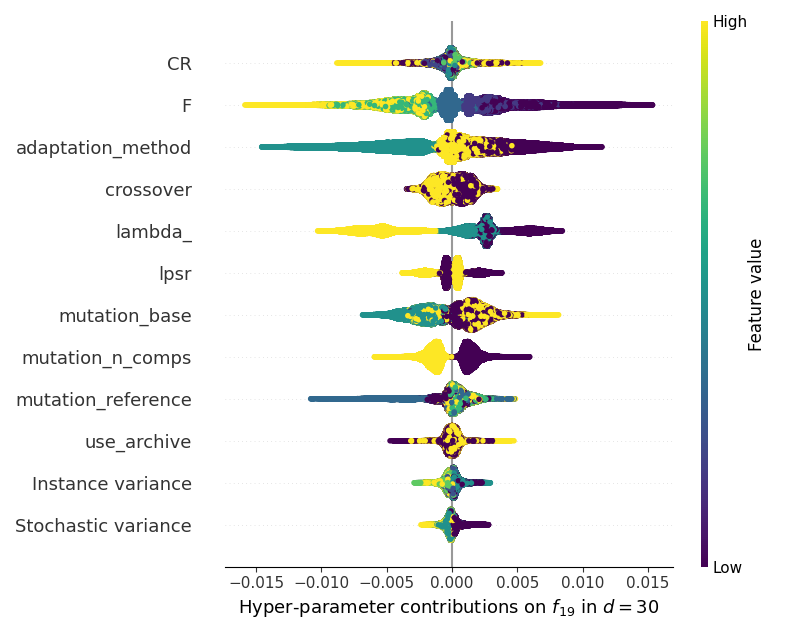
\includegraphics[height=0.15\textheight,trim=60mm 0mm 30mm 0mm,clip]{de_img_new/img_summary_f19_d30.png}
	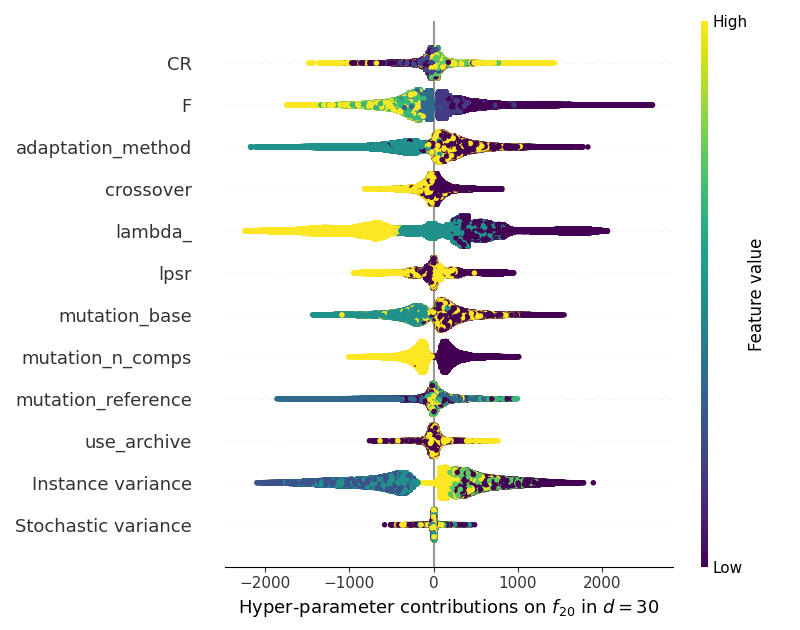
\includegraphics[height=0.15\textheight,trim=60mm 0mm 0mm 0mm,clip]{de_img_new/img_summary_f20_d30.png}
	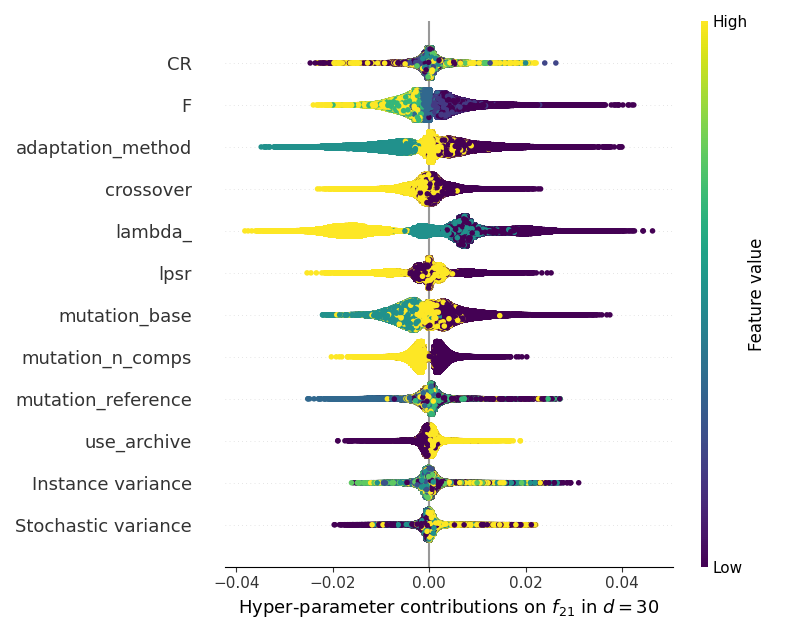
\includegraphics[height=0.15\textheight,trim=0mm 0mm 30mm 0mm,clip]{de_img_new/img_summary_f21_d30.png}
	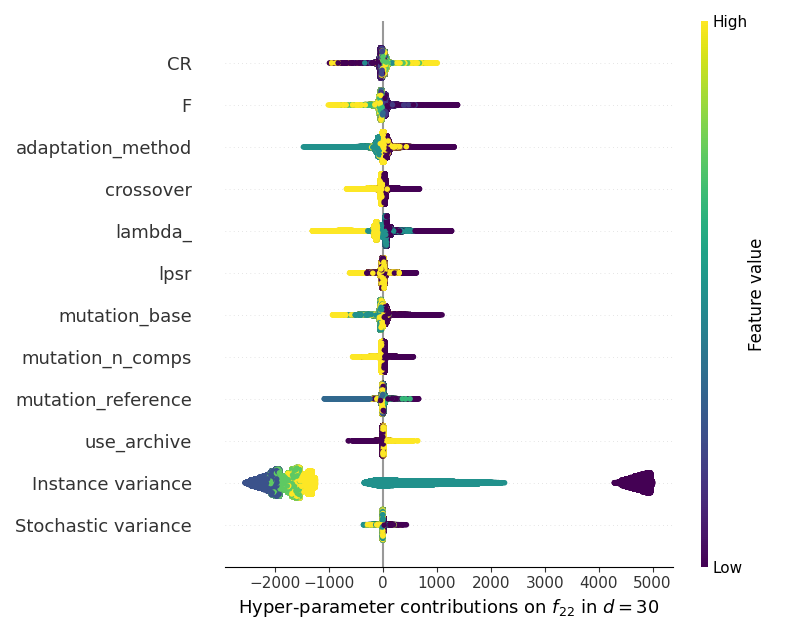
\includegraphics[height=0.15\textheight,trim=60mm 0mm 30mm 0mm,clip]{de_img_new/img_summary_f22_d30.png}
	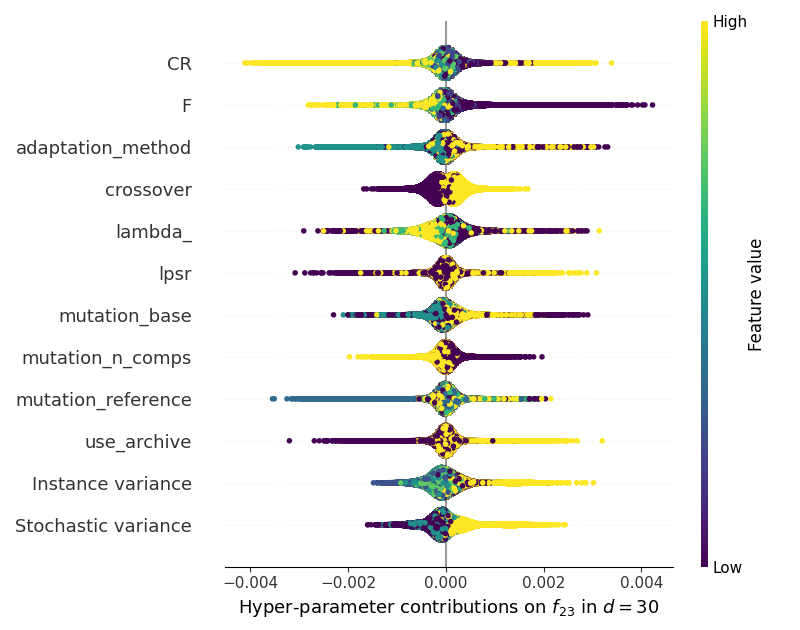
\includegraphics[height=0.15\textheight,trim=60mm 0mm 30mm 0mm,clip]{de_img_new/img_summary_f23_d30.png}
	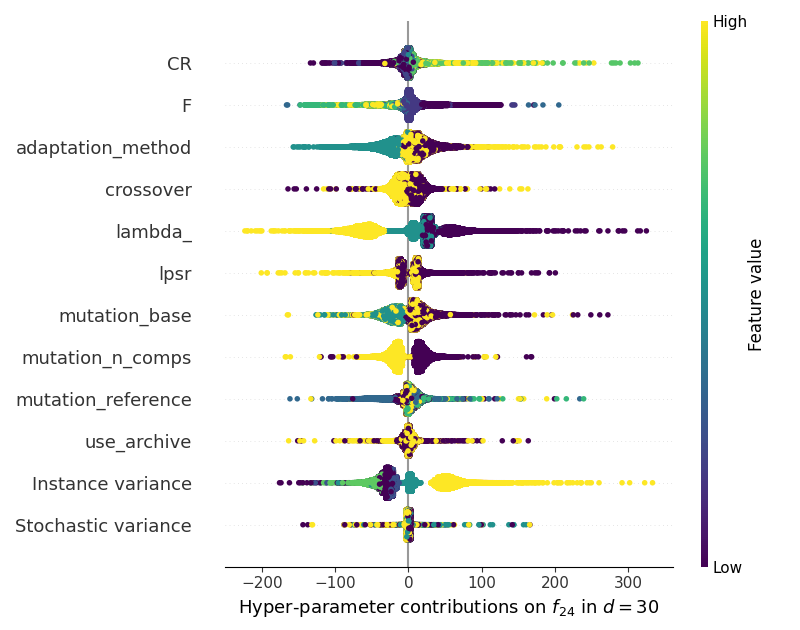
\includegraphics[height=0.15\textheight,trim=60mm 0mm 0mm 0mm,clip]{de_img_new/img_summary_f24_d30.png}
\caption{Hyper-parameter contributions per benchmark function for d=30. \label{fig:shapxplaind30}}

\end{figure}

% Performance stats per dimension and function for mod-DE. Boldface for the single-best configuration indicates a significant improvement over the average best configuration (for that dimension), Boldface for the average best configuration indicates a significant improvement over the average AUC of all configurations.
\begin{table}
\caption{Performance of single-best, average best and average algorithm performance over all configurations per function and dimension.}
\begin{tabular}{llllllll}
\toprule
\multicolumn{4}{c}{d=5} & \multicolumn{4}{c}{d=30} \\
Function & single-best & avg-best & all & Function & single-best & avg-best & all \\
\midrule
f1 Sphere & 0.97 (0.03) & 0.94 (0.08) & 0.81 (0.25) & f1 Sphere & 0.74 (0.32) & \textbf{0.73 (0.31)} & 0.56 (0.25) \\
f2 Ellipsoid & \textbf{0.97 (0.03)} & \textbf{0.93 (0.06)} & 0.69 (0.26) & f2 Ellipsoid & 0.69 (0.20) & \textbf{0.67 (0.19)} & 0.16 (0.13) \\
f3 Rastrigin & \textbf{0.89 (0.07)} & \textbf{0.74 (0.19)} & 0.57 (0.25) & f3 Rastrigin & 0.51 (0.23) & \textbf{0.48 (0.25)} & 0.36 (0.13) \\
f4 BuecheRastrigin & \textbf{0.85 (0.09)} & \textbf{0.70 (0.22)} & 0.52 (0.24) & f4 BuecheRastrigin & 0.48 (0.22) & \textbf{0.47 (0.24)} & 0.33 (0.11) \\
f5 LinearSlope & \textbf{1.00 (0.00)} & 0.99 (0.00) & 0.96 (0.11) & f5 LinearSlope & \textbf{0.97 (0.00)} & \textbf{0.79 (0.12)} & 0.55 (0.22) \\
f6 AttractiveSector & 0.78 (0.15) & \textbf{0.72 (0.18)} & 0.43 (0.20) & f6 AttractiveSector & 0.46 (0.24) & \textbf{0.45 (0.23)} & 0.23 (0.11) \\
f7 StepEllipsoid & \textbf{0.93 (0.01)} & \textbf{0.91 (0.02)} & 0.51 (0.18) & f7 StepEllipsoid & 0.38 (0.01) & \textbf{0.38 (0.01)} & 0.32 (0.02) \\
f8 Rosenbrock & 0.83 (0.12) & \textbf{0.82 (0.12)} & 0.52 (0.25) & f8 Rosenbrock & 0.54 (0.26) & \textbf{0.54 (0.25)} & 0.24 (0.13) \\
f9 RosenbrockRotated & 0.78 (0.09) & \textbf{0.70 (0.19)} & 0.42 (0.19) & f9 RosenbrockRotated & 0.46 (0.22) & \textbf{0.45 (0.21)} & 0.22 (0.09) \\
f10 EllipsoidRotated & 0.88 (0.09) & \textbf{0.79 (0.22)} & 0.37 (0.25) & f10 EllipsoidRotated & \textbf{0.22 (0.02)} & \textbf{0.18 (0.01)} & 0.10 (0.04) \\
f11 Discus & \textbf{0.82 (0.10)} & \textbf{0.61 (0.26)} & 0.32 (0.21) & f11 Discus & \textbf{0.46 (0.19)} & \textbf{0.20 (0.01)} & 0.17 (0.05) \\
f12 BentCigar & 0.74 (0.30) & \textbf{0.68 (0.26)} & 0.34 (0.26) & f12 BentCigar & 0.49 (0.18) & \textbf{0.49 (0.18)} & 0.04 (0.07) \\
f13 SharpRidge & 0.67 (0.27) & 0.61 (0.31) & 0.52 (0.25) & f13 SharpRidge & 0.55 (0.26) & \textbf{0.55 (0.26)} & 0.32 (0.08) \\
f14 DifferentPowers & 0.90 (0.12) & 0.78 (0.29) & 0.75 (0.29) & f14 DifferentPowers & 0.75 (0.31) & \textbf{0.75 (0.30)} & 0.62 (0.25) \\
f15 RastriginRotated & 0.64 (0.31) & 0.57 (0.27) & 0.50 (0.23) & f15 RastriginRotated & 0.37 (0.09) & \textbf{0.34 (0.02)} & 0.31 (0.02) \\
f16 Weierstrass & 0.79 (0.27) & 0.70 (0.28) & 0.69 (0.29) & f16 Weierstrass & 0.75 (0.32) & 0.69 (0.29) & 0.65 (0.29) \\
f17 Schaffers10 & 0.67 (0.29) & 0.64 (0.31) & 0.62 (0.29) & f17 Schaffers10 & 0.63 (0.31) & 0.63 (0.31) & 0.56 (0.26) \\
f18 Schaffers1000 & 0.64 (0.30) & 0.63 (0.30) & 0.58 (0.27) & f18 Schaffers1000 & 0.61 (0.29) & 0.56 (0.26) & 0.48 (0.21) \\
f19 GriewankRosenbrock & 0.76 (0.30) & 0.75 (0.32) & 0.73 (0.30) & f19 GriewankRosenbrock & 0.75 (0.32) & 0.75 (0.32) & 0.71 (0.30) \\
f20 Schwefel & 0.87 (0.17) & \textbf{0.74 (0.26)} & 0.57 (0.26) & f20 Schwefel & 0.71 (0.32) & \textbf{0.67 (0.29)} & 0.30 (0.18) \\
f21 Gallagher101 & 0.89 (0.16) & 0.73 (0.29) & 0.64 (0.27) & f21 Gallagher101 & 0.69 (0.28) & 0.63 (0.28) & 0.53 (0.26) \\
f22 Gallagher21 & 0.83 (0.16) & \textbf{0.76 (0.27)} & 0.59 (0.29) & f22 Gallagher21 & 0.61 (0.33) & 0.60 (0.32) & 0.52 (0.27) \\
f23 Katsuura & 0.79 (0.27) & 0.77 (0.29) & 0.77 (0.28) & f23 Katsuura & 0.78 (0.28) & 0.77 (0.29) & 0.77 (0.28) \\
f24 LunacekBiRastrigin & 0.50 (0.26) & 0.49 (0.26) & 0.48 (0.23) & f24 LunacekBiRastrigin & 0.37 (0.09) & \textbf{0.33 (0.01)} & 0.32 (0.01) \\
\bottomrule
\end{tabular}
\end{table}
% Behaviour stats per dimension and function for mod-DE
\begin{table}
\caption{Algorithm stability of mod-DE}
\begin{tabular}{lrlr}
\toprule
\multicolumn{2}{c}{d=5} & \multicolumn{2}{c}{d=30} \\
Measure & value & Measure & value \\
\midrule
Algorithm stability & -0.02 & Algorithm stability & 0.07 \\
Invar. avg. best & 0.10 & Invar. avg. best & 0.02 \\
S-inv. avg. best & 0.11 & S-inv. avg. best & 0.02 \\
I-inv. avg. best & 0.10 & I-inv. avg. best & 0.01 \\
Invar. single best & 0.43 & Invar. single best & 0.24 \\
S-inv. single best & 0.11 & S-inv. single best & 0.02 \\
I-inv. single best & 0.10 & I-inv. single best & 0.01 \\
Average norm. perf. & 0.58 & Average norm. perf. & 0.39 \\
Gain avg. best & 0.16 & Gain avg. best & 0.16 \\
Gain single best & 0.23 & Gain single best & 0.19 \\
sig. impr. avg best & 1.00 & sig. impr. avg best & 1.00 \\
sig. impr. s. best vs avg best & 1.00 & sig. impr. s. best vs avg best & 0.00 \\
\bottomrule
\end{tabular}
\end{table}
